\chapter{Observations, Curvature, and the Cosmological Fit}

Observational cosmology does not begin, in this lecture, as a list of astronomical facts. It begins by returning to the fundamental equations and asking what an observation could possibly mean once the expansion law and the geometry of space are fixed. We therefore start with the Friedmann equation, the meaning of the Hubble function, and the three FRW spatial geometries; only then do we ask what is actually measured, how the older open-universe picture arose, why dark matter was the first major correction, and how luminosity and number counts as functions of redshift are turned into a fit for the modern values of the \(\Omega\)'s. These notes follow Leonard Susskind's lecture closely, with supporting lecture-board evidence preserved from LazyingArt LLC and Video2Book where it helps fix the mathematical payload.

\section{Friedmann Equation, Hubble Function, and FRW Geometry}

The lecture opens with a methodological point: observational facts have to be placed back into the cosmological equations, otherwise they are not yet cosmology. For a homogeneous universe, the basic equation is
\begin{equation}
H(t)^2
=
\left(\frac{\dot a(t)}{a(t)}\right)^2
=
\frac{8\pi G}{3}\rho(t)-\frac{k}{a(t)^2}.
\end{equation}
Here
\begin{equation}
H(t)=\frac{\dot a(t)}{a(t)}
\end{equation}
is the Hubble function. Susskind pauses over the terminology. One may speak of the \emph{Hubble constant} if one means the value of \(H(t)\) today, but the quantity itself is time-dependent. Throughout the chapter we will denote the present value by \(H_0\).

The curvature parameter is normalized so that
\begin{equation}
k\in\{+1,0,-1\},
\end{equation}
with \(k=+1\) for spherical spatial geometry, \(k=0\) for flat space, and \(k=-1\) for hyperbolic space.

The scale factor \(a(t)\) enters the metric directly. The lecture writes the metric in the usual FRW form, with the angular part compressed into a single function \(\xi(r)\):
\begin{equation}
ds^2
=
-dt^2+a(t)^2\left[dr^2+\xi(r)^2\,d\Omega_2^2\right],
\end{equation}
where
\begin{equation}
\xi(r)=
\begin{cases}
\sin r, & k=+1,\\[4pt]
r, & k=0,\\[4pt]
\sinh r, & k=-1.
\end{cases}
\end{equation}
This notation is useful later, because the same \(\xi(r)\) that describes the metric also controls the growth of areas and shell volumes, and therefore enters directly into observable counting formulas.

At this stage the lecture has fixed the stage completely: three possible spatial geometries and one dynamical variable \(a(t)\). Everything that follows is an attempt to connect these ingredients to things astronomers can actually observe.

\section{What Enters the Equation Today, and What Astronomers Can Measure}

The next move is to decompose the energy density into the pieces relevant for the present universe. In the lecture the right-hand side is written as a bookkeeping sum of radiation, matter, vacuum energy, and curvature:
\begin{equation}
\frac{C_r}{a^4}+\frac{C_m}{a^3}+\Lambda-\frac{k}{a^2}=H^2.
\end{equation}
The constants \(C_r\) and \(C_m\) are time-independent normalizations. Radiation dilutes as \(a^{-4}\), nonrelativistic matter as \(a^{-3}\), vacuum energy does not dilute at all, and the curvature term scales as \(a^{-2}\).

\begin{definition}
The present-day density parameters are defined by dividing each of these terms, evaluated today, by \(H_0^2\). Thus
\begin{equation}
\Omega_r+\Omega_m+\Omega_\Lambda+\Omega_k=1,
\end{equation}
with
\begin{equation}
\Omega_k=\frac{-k/a_0^2}{H_0^2},
\end{equation}
where \(a_0=a(t_{\mathrm{today}})\).
\end{definition}

The point of this decomposition is operational. Once we write the four terms on the board, the next question is immediate: how much of \(H_0^2\) comes from radiation, how much from matter, how much from vacuum energy, and how much is left to curvature?

The Hubble term is measured by the relation between redshift and distance. In the original Hubble construction, redshift gave velocity and brightness gave distance. The lecture insists on the practical point that the early measurements were local enough that Hubble was really measuring the present value \(H_0\), not tracing the time-dependence of \(H(t)\) deep into the past.

Radiation is easier. Today it is dominated by the cosmic microwave background, and its energy density is tiny compared with matter. One does not need very deep cosmology to know that \(\Omega_r\) is very small at present.

Matter is then estimated by adding up the luminous content of galaxies: stars, gas, hydrogen, and the ordinary visible baryonic inventory. The lecture quotes the rough scale as about one proton per cubic meter on average. This is a very low density, but still much larger than the radiation energy density today.

\subsection{Question \& Answer}

A natural objection appears immediately: how can brightness be used as a distance indicator if distant objects are not all intrinsically identical?

The lecture answers by invoking the cosmic distance ladder. One does not assume all sources have the same luminosity. Instead, one chains together overlapping standards. The nearest stars are calibrated by parallax. Among those nearby stars one identifies Cepheid variables, whose period-luminosity relation provides a standard candle. That standard candle can then be exported to greater distances. Higher still on the ladder, supernovae become the best standard candles for the redshifts relevant to cosmology. In other words, distance is not guessed from raw brightness; it is inferred from brightness only after a ladder of overlapping calibrations has been built.

This exchange matters for the logic of the lecture. Brightness is not introduced as a textbook definition, but as a measurement that has first earned the right to be trusted.

\section{The Older Cosmological Picture and Why It Seemed to Favor an Open Universe}

Susskind then deliberately steps into the historical viewpoint. We are to imagine the old cosmological bookkeeping before dark matter and before the return of \(\Lambda\) as a serious cosmological term. In that picture,
\begin{equation}
\Omega_r \approx 0,\qquad \Omega_\Lambda=0,
\end{equation}
and \(\Omega_m\) was taken from luminous matter alone, hence was believed to be small.

\begin{figure}
\centering

\includegraphics[width=0.72\textwidth]{lecture_06_figure_02.png}
\caption{Board review of the matter-era relation between \(a(t)\) and the Hubble scale. The frame is cropped, so the clean equations are written explicitly in the text.}
\end{figure}

The bridge between Friedmann dynamics and cosmic age is the matter-dominated solution
\begin{equation}
a(t)\propto t^{2/3}.
\end{equation}
From this one obtains
\begin{equation}
\dot a(t)\propto \frac{2}{3}t^{-1/3},
\end{equation}
and therefore
\begin{equation}
\frac{\dot a}{a}=\frac{2}{3t}.
\end{equation}
So in a matter-dominated universe,
\begin{equation}
H(t)=\frac{2}{3t},
\end{equation}
and in particular
\begin{equation}
H_0\sim \frac{1}{T},
\end{equation}
where \(T\) is the age of the universe, up to the factor \(2/3\).

This is the first worked derivation of the lecture, and it does real conceptual work. The Hubble scale is not merely an astronomer's unit of kilometers per second per megaparsec; in the matter-dominated approximation it is essentially the inverse age of the universe.

Susskind briefly compares this with the radiation-dominated case,
\begin{equation}
a(t)\propto t^{1/2},
\qquad
H(t)=\frac{1}{2t},
\end{equation}
to emphasize the broader point: for simple equations of state, the Hubble scale today is generically of order the inverse cosmic age.

From the old observational standpoint, the matter term inferred from luminous matter was too small to account for \(H_0^2\). The gap was of order twenty to thirty. Therefore, in the old accounting, the curvature term had to do most of the work:
\begin{equation}
-\frac{k}{a_0^2}\sim H_0^2.
\end{equation}
This immediately forced the sign
\begin{equation}
k<0,
\end{equation}
since the curvature contribution had to be positive on the right-hand side.

Thus the old cosmological picture pointed toward an open, negatively curved universe. Combining the two rough relations,
\begin{equation}
\frac{1}{a_0^2}\sim H_0^2,
\qquad
H_0\sim \frac{1}{T},
\end{equation}
one arrived at the historical conclusion that the curvature radius was of order the age of the universe. In units with \(c=1\), age and length can be directly compared; in ordinary units this means a radius of curvature of order \(cT\).

This is not the modern conclusion, and the lecture says so explicitly. But it is important to see why it once looked unavoidable.

\section{Dark Matter as the First Correction: Rotation Curves and Galactic Halos}

The first serious correction to this older picture was dark matter. The lecture introduces it by slowing down and asking a very concrete Newtonian question: how do stars move in galaxies?

The starting point is the old assumption that most of the luminous mass lies near the galactic center. If so, an outer star should move under the influence of an approximately central mass \(M\). The transcript becomes garbled during part of the board derivation, so here we write the standard force-balance equation in cleaned form:
\begin{equation}
\frac{GM}{r^2}=\frac{v^2}{r}.
\end{equation}
Multiplying by \(r\), we find
\begin{equation}
v^2=\frac{GM}{r},
\end{equation}
and therefore
\begin{equation}
v(r)\propto r^{-1/2}.
\end{equation}
This is the Kepler-law expectation: orbital speed should fall as the inverse square root of radius.

\begin{figure}
\centering

\includegraphics[width=0.78\textwidth]{lecture_06_figure_03.png}
\caption{Board evidence for the central-force setup used in the galaxy rotation-curve argument. Only the numerator \(MG\) and the fraction bar are fully visible in the frame; the completed equation is reconstructed from the lecture's argument.}
\end{figure}

\begin{figure}
\centering
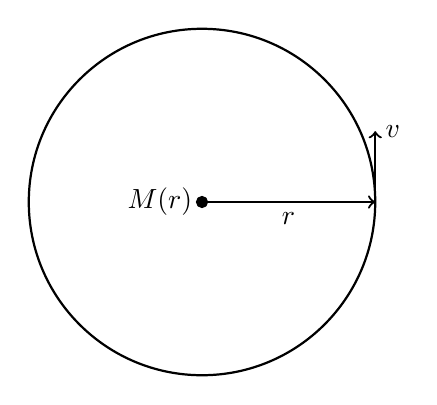
\begin{tikzpicture}[scale=1.0]
\draw[thick] (0,0) circle (2.2);
\filldraw (0,0) circle (2pt);
\draw[->,thick] (0,0)--(2.2,0) node[midway,below] {$r$};
\draw[->,thick] (2.2,0)--(2.2,0.9) node[right] {$v$};
\node[left] at (0,0) {$M(r)$};
\end{tikzpicture}
\caption{Clean reconstruction of the orbit sketch behind the rotation-curve calculation. The enclosed gravitating mass may depend on the orbital radius.}
\end{figure}

But that is not what is observed. The rotation curves are approximately flat. The outer stars do not slow down as \(r^{-1/2}\).

So the lecture replaces the central mass \(M\) by an enclosed mass \(M(r)\), the total gravitating mass inside radius \(r\). Then the force-balance equation becomes
\begin{equation}
\frac{G\,M(r)}{r^2}=\frac{v^2}{r}.
\end{equation}
If the observed velocity is roughly constant, then
\begin{equation}
v(r)\approx \mathrm{const},
\end{equation}
and therefore
\begin{equation}
M(r)\propto r.
\end{equation}
This is the key inference. The enclosed gravitating mass continues to grow with radius far beyond the region in which the luminous matter is concentrated.

The lecture is careful here. This does not mean the \emph{density} is linear in \(r\); it means the total enclosed mass is. The conclusion is that there is more gravitating matter than luminous matter, distributed in an extended halo.

The same style of evidence appears on multiple scales: galaxies, interactions among galaxies, and clusters of galaxies. The simplest reading is that there is a large non-luminous mass component.

\subsection{Question \& Answer}

Once this is accepted, the next question arises naturally: why did the dark matter not collapse into the same visible disk as the luminous matter?

The lecture's answer is dynamical, not metaphysical. Ordinary luminous matter is made of electrically charged particles. It collides, radiates, and dissipates energy. Because it can lose energy efficiently, it collapses into a thinner, more centrally concentrated structure. Dark matter, by contrast, appears to be much more weakly interacting. In particular, it is not electrically charged, so it does not radiate electromagnetically. Its particles can orbit, stream through one another, and remain in a large halo because there is no efficient dissipative channel to make them settle into the luminous disk. Gravitational-wave emission is far too weak to play this role.

The halo is therefore expected to remain extended and approximately spherical. It may be denser near the galactic center, but it need not mimic the visible morphology of the galaxy.

The lecture also stresses a second qualitative property: the dark matter must be cold enough to cluster strongly. Neutrinos, being too light and hence too fast, behave as hot dark matter and do not provide a good fit to the observed clustering. Various particle candidates remain possible, including bosonic condensate pictures such as axions, but the lecture does not attempt to settle the particle-physics model.

\section{Why Dark Matter Still Does Not Fix the Old Friedmann Budget}

Dark matter enlarges the matter term, but it does not by itself repair the old curvature-dominated picture. This point is important because otherwise one might imagine that adding unseen mass simply closes the old gap and ends the story.

That is not what happened. If the luminous matter had originally undershot the required value by a factor of roughly \(20\) to \(30\), and dark matter adds only a factor of order \(5\) to \(10\), then the matter term still does not account for \(H_0^2\):
\begin{equation}
\frac{C_m}{a_0^3}\not\approx H_0^2.
\end{equation}
It becomes larger than the luminous contribution alone, but not large enough to eliminate the need for the curvature term in the older model. In that sense dark matter was a major correction, but not yet the final one.

This is why the lecture now pivots away from mere contents. The question becomes sharper: if we have a candidate cosmology, how do we actually test it as a whole?

\section{How a Cosmological Model Is Tested: Geometry, Redshift, and Number Counts}

A model, in the lecture's language, consists of two things: a value of \(k\), and an equation of state, or equivalently an expansion history \(a(t)\). That is the level at which a cosmology is to be tested.

\begin{figure}
\centering

\includegraphics[width=0.72\textwidth]{lecture_06_figure_04.png}
\caption{Context frame for the lecture's transition from contents to models. The visible \(k=0\) and probable \(\xi=r\) belong to the flat case, while the cropped right board preserves the Hubble/Friedmann structure only schematically.}
\end{figure}

The lecture first freezes the time-dependence and asks a purely geometric question: if space were static, how would counts and brightness reveal curvature?

In a shell of thickness \(dr\), the number of galaxies is proportional to the shell area times \(dr\). Because the shell area scales as \(\xi(r)^2\), one has
\begin{equation}
dN\propto \xi(r)^2\,dr.
\end{equation}
Thus, in flat space,
\begin{equation}
dN\propto r^2\,dr,
\end{equation}
whereas in negatively curved space,
\begin{equation}
dN\propto \sinh^2 r\,dr\sim e^{2r}\,dr
\qquad
(r\ \text{large}).
\end{equation}
So negative curvature causes the number of objects in successive shells to grow anomalously quickly with distance.

Likewise, in flat space the observed flux from a source falls with the inverse area of the sphere surrounding it:
\begin{equation}
F\propto \frac{1}{r^2}.
\end{equation}
In negatively curved space the area of spheres grows faster than \(r^2\), so the apparent brightness falls faster with distance. In the lecture this is described somewhat loosely in terms of luminosity, but physically it is the observed flux that carries the inverse-area dependence.

Now the time-dependence is restored. We do not see a large spatial slice all at once. We look outward by looking backward in time along incoming light rays. If light is emitted with wavelength \(\lambda_{\mathrm{em}}\) and observed today with wavelength \(\lambda_{\mathrm{obs}}\), then the expansion stretches the wavelength by the ratio of scale factors:
\begin{equation}
1+z=\frac{\lambda_{\mathrm{obs}}}{\lambda_{\mathrm{em}}}=\frac{a_0}{a(t_{\mathrm{em}})}.
\end{equation}
The redshift \(z\) is defined by
\begin{equation}
z=\frac{\lambda_{\mathrm{obs}}}{\lambda_{\mathrm{em}}}-1.
\end{equation}

To connect redshift with distance, we need the motion of radial light rays. For radial null rays, \(d\Omega_2=0\) and \(ds^2=0\), so the metric gives
\begin{equation}
dt^2=a(t)^2\,dr^2.
\end{equation}
For the past-directed incoming branch, we choose
\begin{equation}
dt=-a(t)\,dr,
\qquad\text{or equivalently}\qquad
\frac{dr}{dt}=-\frac{1}{a(t)}.
\end{equation}

\begin{figure}
\centering

\includegraphics[width=0.84\textwidth]{lecture_06_figure_05.png}
\caption{Board bridge between the observable side, centered on \(dN/dz\), and the model side, centered on \(a(t)\), \(\dot a(t)\), and \(r(t)\).}
\end{figure}

\paragraph{A cleaned derivation of \(\boldsymbol{dN/dz}\).}
The lecture derives this formula live, and the algebra on the board is halting and self-correcting. The clean structure is nevertheless straightforward. Start from
\begin{equation}
dN\propto \xi(r)^2\,dr.
\end{equation}
Differentiate the redshift relation:
\begin{equation}
1+z=\frac{a_0}{a}
\quad\Longrightarrow\quad
dz=-\frac{a_0}{a^2}\,da.
\end{equation}
Now write
\begin{equation}
da=\dot a\,dt,
\end{equation}
and along the incoming null ray use
\begin{equation}
dt=-a\,dr.
\end{equation}
Therefore
\begin{equation}
dz
=
-\frac{a_0}{a^2}\dot a\,dt
=
-\frac{a_0}{a^2}\dot a\,(-a\,dr)
=
\frac{a_0}{a}\dot a\,dr
=
(1+z)\dot a\,dr.
\end{equation}
So
\begin{equation}
dr=\frac{dz}{(1+z)\dot a},
\end{equation}
and hence
\begin{equation}
\frac{dN}{dz}\propto \frac{\xi(r)^2}{(1+z)\dot a}.
\end{equation}

\begin{remark}
This is the cleaned outcome of the lecture's board derivation, not a claim that the live algebra was presented in polished form. The pedagogical point in the lecture is precisely that once a model determines \(a(t)\), it also determines \(\dot a(t)\), the null-ray trajectory \(r(t)\), and therefore the observable count \(dN/dz\).
\end{remark}

This is the key bridge from theory to observation. Geometry enters through \(\xi(r)\). Expansion enters through \(a(t)\) and \(\dot a(t)\). Redshift ties them together.

\section{From Trial Parameters to the Best Fit Universe}

Once the bridge to observables has been built, the fitting logic becomes almost algorithmic. One chooses trial values for the present-day density parameters, solves the Friedmann equation, computes the observables, and compares them with data.

\begin{figure}
\centering

\includegraphics[width=0.84\textwidth]{lecture_06_figure_06.png}
\caption{Summary board for the matter-dominated negative-curvature model under test. The boxed equation specializes Friedmann to matter plus curvature, while the lower board retains the shell-growth reminders \(r^2dr\) and \(e^{2r}dr\).}
\end{figure}

The older model under discussion may be summarized as
\begin{equation}
\frac{C_m}{a^3}-\frac{k}{a^2}=H^2,
\end{equation}
with \(k<0\), matter domination, and no cosmological constant. Once one chooses such a model, one computes \(a(t)\), then \(r(t)\), then the predicted relations \(L(z)\) and \(dN/dz\). This model fails. It does not reproduce the observed brightness-redshift relation, nor the observed number counts.

The data instead favor the modern fit
\begin{equation}
\Omega_r\approx 0,\qquad
\Omega_m\approx 0.3,\qquad
\Omega_\Lambda\approx 0.7,\qquad
\Omega_k\approx 0.
\end{equation}
The matter fraction here includes both luminous matter and dark matter.

Supernovae provide the best standard candles at the redshifts of interest, so the luminosity-redshift relation is effectively a supernova test. The lecture also notes that the cosmic microwave background supplies an independent triangulation of curvature, and that the percent-level statement \(\Omega_k\approx 0\) is sharpened substantially when supernova information is supplemented with CMB data.

\subsection{Question \& Answer}

A persistent question arises at the end of the lecture: what is actually measured directly, what is inferred by fitting, and why does only one late-time trial parameter remain effectively free?

The clean answer is this. Radiation is negligible today and is known to be small directly. The matter fraction \(\Omega_m\) is approximately measurable from the matter density and \(H_0\), provided one includes the dark matter contribution inferred from gravitational evidence. The sum rule
\begin{equation}
\Omega_r+\Omega_m+\Omega_\Lambda+\Omega_k=1
\end{equation}
then relates the remaining unknown pieces. So at late times, once \(\Omega_r\) is negligible and \(\Omega_m\) is approximately fixed, one may take \(\Omega_\Lambda\) as a trial parameter and let \(\Omega_k\) be whatever is required to fill out the sum. But that does \emph{not} mean \(\Omega_k\) is ignored. It still affects the predicted observables through the Friedmann solution and the geometry function \(\xi(r)\). A bad trial value of \(\Omega_\Lambda\) forces a bad implied \(\Omega_k\), and the resulting model fails when compared with \(L(z)\) and \(dN/dz\).

So the logic is not that \(\Omega_\Lambda\) is directly measured from a single equation. The logic is:
\begin{enumerate}
\item choose trial present-day parameters,
\item solve Friedmann,
\item compute observables,
\item compare with the data,
\item reject or keep the model.
\end{enumerate}

The lecture insists on one final conceptual point. The \(\Omega\)'s are defined using \emph{today's} values, so they are not constants of time. Long in the past, because the radiation term scales as \(a^{-4}\), one had
\begin{equation}
\Omega_r\approx 1.
\end{equation}
Later matter rose to dominance. In the far future, if \(\Lambda\) continues to dominate,
\begin{equation}
\Omega_\Lambda\to 1.
\end{equation}
The matter fraction therefore starts small, becomes large, and then decreases again. The curvature fraction is consistent with zero today only at about the percent level, not exactly. If the universe keeps expanding, the large-scale geometry becomes effectively flatter and flatter in the sense that the curvature term becomes ever less important compared with the cosmological-constant term. Susskind's short phrase is memorable: big is flat.

The final emphasis of the lecture is methodological. We are not merely testing a preferred model. We are testing a model by feeding it through the governing equations and asking whether the resulting observables match the sky at all.

\section{Summary}

The lecture begins by refusing to separate observation from dynamics. Once the Friedmann equation and FRW geometry are restored, the present-day cosmic budget can be organized into radiation, matter, vacuum energy, and curvature, and the older open-universe picture can be reconstructed from the smallness of luminous matter alone. Dark matter enters first through a concrete Newtonian failure of Kepler falloff in galaxy rotation curves, and it corrects the matter budget without fully repairing the old curvature-dominated model.

The decisive step is then to convert a cosmological model into observables. Geometry controls shell growth through \(\xi(r)\); expansion controls redshift and null propagation through \(a(t)\); together they determine the luminosity-redshift relation and the count \(dN/dz\). The matter-dominated \(k<0\) model fails this test. The modern fit,
\[
\Omega_m\approx 0.3,\qquad
\Omega_\Lambda\approx 0.7,\qquad
\Omega_k\approx 0,
\]
succeeds at the percent level. The broader lesson is that observational cosmology is not a catalogue of numbers. It is the disciplined comparison of data with the consequences of the Friedmann equations.